\documentclass[tikz, border=10pt]{standalone}
\usetikzlibrary{arrows.meta,calc}

\begin{document}
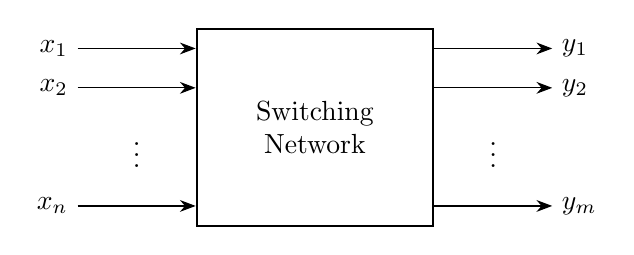
\begin{tikzpicture}[
    box/.style={rectangle, draw, thick, minimum height=2.5cm, minimum width=3cm, align=center},
    line/.style={draw, -{Stealth[length=2mm]}}
]
    % Switching network block
    \node[box] (network) {Switching \\ Network};

    % Inputs
    \foreach \y/\label in {1/x_1, 0.5/x_2, -1/x_n} {
        \draw[line] (network.west) ++(-1.5, \y) node[left] {$\label$} -- ++(1.5, 0);
    }
    \node at ($(network.west) + (-0.75, -0.25)$) {$\vdots$};

    % Outputs
    \foreach \y/\label in {1/y_1, 0.5/y_2, -1/y_m} {
        \draw[line] (network.east) ++(0, \y) -- ++(1.5, 0) node[right] {$\label$};
    }
    \node at ($(network.east) + (0.75, -0.25)$) {$\vdots$};

\end{tikzpicture}
\end{document}
